\documentclass{beamer}

% Metadata
\title{Statische Typsysteme für JavaScript}
\subtitle{Entwicklung eines Transpilers zur Übersetzung von Flow nach TypeScript}
\author{Jonathan Gruber}
\institute{HTWK Leipzig}
\date{18. Dezember 2019}

% Encoding
\usepackage[utf8]{inputenc}
\usepackage[T1]{fontenc}

% Babel
\usepackage[ngerman]{babel}

% Fonts
\usepackage{arev} % for Math
\usepackage[sb]{plex-sans}
\usepackage[scale=0.8,sb]{plex-mono}

% Biber (references)
\usepackage[backend=biber]{biblatex}
\addbibresource{src/references.bib}

\let\OLDitemize\itemize
\renewcommand\itemize{\OLDitemize\addtolength{\itemsep}{4pt}}

\let\OLDenumerate\enumerate
\renewcommand\enumerate{\OLDenumerate\addtolength{\itemsep}{2pt}}

\usepackage{csquotes}
\usepackage{longtable, tabu, booktabs}
\usepackage{tikz}
\usepackage{hyperref}

% Code listings
\usepackage{listings}

\lstset{
  aboveskip=0pt,
  basicstyle=\linespread{1.04}\small\ttfamily,
  belowcaptionskip=0pt,
  belowskip=0pt,
  breakatwhitespace=true,
  breaklines=true,
  comment=[l]{//},
  commentstyle=\color{darkgray},
  emph={?, any, Array, boolean, empty, interface, mixed, never, number, null, opaque, string, this, unknown, void, T, TypeAlias},
  emphstyle=\itshape,
  extendedchars=false,
  keywords={abstract, arguments, await, boolean, break, byte, case, catch, char, class, const, continue, debugger, declare, default, delete, do, double, else, enum, eval, export, extends, false, final, finally, float, for, function, goto, if, implements, import, in, instanceof, int, let, long, module, native, new, of, package, private, protected, public, return, short, static, super, switch, synchronized, this, throw, throws, transient, true, try, typeof, var, volatile, while, with, yield, type},
  keywordstyle=\bfseries,
  morecomment=[s]{/*}{*/},
  morestring=[b]',
  morestring=[b]",
  numbers=left,
  numbersep=12pt,
  numberstyle=\linespread{1.04}\scriptsize\ttfamily\color{gray},
  showspaces=false,
  showstringspaces=false,
  stepnumber=1,
  stringstyle=\color{black},
  tabsize=4,
}

% The following ensures that only straight quotes are used inside of \texttt
\usepackage{upquote}
\usepackage{etoolbox}

\robustify{\texttt}
\let\originaltexttt\texttt

\begingroup
\catcode`'=\active
\catcode``=\active
\globaldefs1
\makeatletter
\renewrobustcmd{\texttt}[1]{%
  {%
  \everyeof{\noexpand}\endlinechar-1
  \expandafter\catcode\string``=\active
  \expandafter\catcode\string`'=\active
  \let'\textquotesingle
  \let`\textasciigrave
  \ifx\encodingdefault\upquote@OTone
    \ifx\ttdefault\upquote@cmtt
    \def'{\char13 }\def`{\char18 }%
    \fi
  \fi
  \scantokens{\originaltexttt{#1}}%
  }%
}%
\endgroup


% Trees
\usepackage{forest,subcaption}

% Style for edge labels
\tikzset{edge/.style = {
  midway,fill=white,font=\scriptsize
}}

\forestset{
  font=\scriptsize,
  default preamble={
    for tree = {
      l=1.5cm,
      s sep=.75cm,
      inner xsep=2mm,
      inner ysep=1.25mm,
      minimum height=4.75mm,
      rectangle,
      rounded corners=2,
      fill=mlightgray,
      font=\scriptsize,
    }
  }
}


% Theme
\definecolor{pcolor}{HTML}{06594f}
\definecolor{scolor}{HTML}{01517f}
\definecolor{mlightgray}{HTML}{DCDCDC}
\usetheme{Frankfurt}
\setbeamercolor{bibliography entry author}{fg=black}
\setbeamercolor{bibliography entry location}{fg=black}
\setbeamercolor{bibliography entry note}{fg=black}
\setbeamercolor{bibliography entry title}{fg=black}
\setbeamercolor{enumerate item}{fg=black}
\setbeamercolor{enumerate subitem}{fg=black}
\setbeamercolor{itemize item}{fg=black}
\setbeamercolor{itemize subitem}{fg=black}
\setbeamerfont{frametitle}{series=\bfseries,parent=structure}
\setbeamertemplate{bibliography item}{\insertbiblabel}
\setbeamertemplate{blocks}[default]
\setbeamertemplate{enumerate items}[default]
\setbeamertemplate{frametitle}[default][shadow=false]
\setbeamertemplate{footline}[frame number]
\setbeamertemplate{itemize items}[circle]
\setbeamertemplate{navigation symbols}{}
\setbeamertemplate{title page}[default][rounded=true,shadow=false]
\usecolortheme[named=pcolor]{structure}

% Remove shadow from navigation bar
\useoutertheme{smoothbars}
\makeatletter
\AtBeginDocument{
\pgfdeclareverticalshading{beamer@barshade}{\the\paperwidth}{%
    color(0ex)=(black);%
    color(0.5ex)=(section in head/foot.bg);%
    color(4ex)=(section in head/foot.bg)%
  }
}

% Small font in bibliography
\renewcommand*{\bibfont}{\small}

% Titlepage
\makeatletter
\setbeamertemplate{title page}
{
  \vfill
  \begin{centering}
    \setbeamercolor{title}{bg=white,fg=black}

    \begin{beamercolorbox}[center]{author}
      \usebeamerfont{author}\normalsize Masterkolloquium
    \end{beamercolorbox}

    \vspace{0.5cm}

    \begin{beamercolorbox}[sep=8pt,center]{title}
      \usebeamerfont{title}{\huge\textbf{Statische Typsysteme\\für JavaScript}}
    \end{beamercolorbox}

    \begin{beamercolorbox}[sep=6pt,center]{title}
      \usebeamerfont{title}\large Entwicklung eines Transpilers zur\\Übersetzung von Flow nach TypeScript
    \end{beamercolorbox}

    \vspace{0.5cm}

    \begin{beamercolorbox}[sep=3pt,center]{author}
      \usebeamerfont{author}\normalsize\insertauthor
    \end{beamercolorbox}

    \begin{beamercolorbox}[sep=3pt,center]{institute}
      \usebeamerfont{institute}{\normalsize\insertinstitute}
    \end{beamercolorbox}

    \vspace{0.5cm}

    \begin{beamercolorbox}[sep=3pt,center]{date}
      \usebeamerfont{date}{\normalsize\insertdate}
    \end{beamercolorbox}
  \end{centering}
  \vfill
}
\makeatother

\newcommand{\pie}[1]{%
	\begin{tikzpicture}%
    \draw[pcolor] (0,0) circle (0.7ex);%
    \fill[rotate=-90,fill=pcolor] (0.7ex,0) arc (0:-#1*180:0.7ex) -- (0,0) -- cycle;%
	\end{tikzpicture}%
}

\newcommand*\circled[1]{
  \tikz[baseline=(char.base)]{
    \node[shape=rectangle,fill=white,text=scolor,inner sep=6pt] (char) {#1};
  }
}

\newcommand{\secframe}[2]{
  {
    \setbeamercolor{background canvas}{bg=scolor}
    \begin{frame}[plain]
      \Huge\color{white}\textbf{\circled{#1}\hspace{0.5em}#2}
    \end{frame}
  }
}


\begin{document}
  \frame[plain]{\titlepage}

  \frame[plain]{
    \frametitle{}
    \LARGE{\textbf{Überblick}}
    \vspace{1em}
    \large
    \begin{enumerate}
      \item Problemstellung
      \item Umsetzung des Transpilers
      \item Ergebnisse und Auswertung
      \item Zusammenfassung
    \end{enumerate}
  }

  \section{Problemstellung}
    \secframe{1}{Problemstellung}

    \begin{frame}
      \frametitle{Motivation}
      \begin{itemize}
        \item JavaScripts \textbf{dynamische Typisierung} erschwert die Entwicklung korrekter, sicherer und wartbarer Anwendungen~\autocite{NIKHIL:2014,PRADEL:2015,BIERMAN:2014}
        \item Typ von Werten wird zur Laufzeit implizit umgewandelt (\textit{type coercion})
        \item Kritisches Laufzeitverhalten wird zum Teil ignoriert
        \item aber: bessere Typsicherheit durch Einsatz eines\\\textbf{statischen Typsystems} möglich
        \item Zwei Vertreter: \textit{Flow}~\autocite{FLOW:PAPER} und \textit{TypeScript}~\autocite{TYPESCRIPT:SPEC}
      \end{itemize}
    \end{frame}

    \begin{frame}[fragile]
      \frametitle{Beispiel -- Statische Typisierung durch Flow}
      \begin{lstlisting}
function linearSearch<T>(list: Array<T>, searchValue: T): number | null {
  for (const [index, value] of list.entries()) {
    if (value === searchValue) {
      return index;
    }
  }
  return null;
}

linearSearch<number>([3, 56, 10], 56);           // 1
linearSearch<number>([3, 56, 10], 12);           // null
linearSearch<string>(['foo', 'bar', 'baz'], 3);  // Typfehler
      \end{lstlisting}
    \end{frame}

    \frame{
      \frametitle{Zielsetzung der Masterarbeit}
      \begin{itemize}
        \item Ausgangslage: \textit{Spreadshirt} setzt Flow zur statischen Typisierung von JavaScript-Anwendungen ein
        \item Ziel: Migration bestehender Flow"=Projekte nach TypeScript
        \item Händische Migration fehleranfällig und zeitaufwändig
        \item Lösung: Entwicklung eines \textbf{Transpilers} zur Übersetzung der Flow-Typisierung nach TypeScript
        \item Transpiler = Compiler, der Quelltext einer Programmier"=sprache in eine andere übersetzt
      \end{itemize}
    }

    \begin{frame}[fragile]
      \frametitle{Beispiel einer Typ-Übersetzung}

      \begin{lstlisting}[
        numbers=none,
        emph={number,null,undefined}
      ]
// Flow
type MaybeNumber = ?number;


// TypeScript
type MaybeNumber = number | null | undefined;
      \end{lstlisting}
    \end{frame}

    \begin{frame}
      \frametitle{Ziele der Migration zu TypeScript}
      \begin{enumerate}
        \item Erkennung weiterer Typ- und Programmfehler
        \item Unterstützung externer Bibliotheken
        \item Performance der Typüberprüfungen
        \item Zukunftssicherheit und Transparenz der Technologie
      \end{enumerate}
    \end{frame}

  \section{Umsetzung}
    \secframe{2}{Umsetzung}

    \begin{frame}
      \frametitle{Technische Anforderungen an den Transpiler}
      \begin{enumerate}
        \item Äquivalente und vollständige Übersetzung der Flow-Typen
        \item Beibehaltung der Programmsemantik
        \item Unterstützung aktueller und vorläufiger JavaScript- sowie JSX-Syntax
        \item Verarbeitung gesamter Projektverzeichnisse
        \item Beibehaltung der Quelltextformatierung
      \end{enumerate}
    \end{frame}

    \begin{frame}
      \frametitle{Implementierung als Babel-Plugin}
      \begin{itemize}
        \item \textit{Babel}~\autocite{BABEL} als Grundlage der Implementierung
        \item Babel = Transpiler für JavaScript
        \item unterstützt alle geforderten Syntaxarten
        \item Erweiterung durch Plugins möglich
        % \item Programmtransformation durch Manipulation des abstrakten Syntaxbaums (AST)
      \end{itemize}
    \end{frame}

    \begin{frame}
      \frametitle{Programmtransformation durch Babel}
      \begin{enumerate}
        \item Parsen des Eingabequelltexts\linebreak$\Rightarrow$ abstrakter Syntaxbaum (AST) des Programms
        \item Programmtransformation durch Manipulation der AST-Knoten mittels \textit{Besucher-Entwurfsmuster}
        \item Generierung des Ausgabequelltexts
      \end{enumerate}
    \end{frame}

    \begin{frame}[fragile]
      \frametitle{Transformation des AST}

      \begin{columns}
        \begin{column}{.48\textwidth}
          \begin{lstlisting}[numbers=none]
// @flow
type Alias = mixed;
          \end{lstlisting}
          \vspace{5mm}
          \ttfamily
          \begin{forest}
            for tree = {l=1.6cm, s sep=0.4cm}
            [Program
              [TypeAlias, edge label={node[edge]{body}}
                [Identifier, edge label={node[edge]{id}}
                  [\enquote{Alias}, edge label={node[edge]{name}}]
                ]
                [MixedTypeAnnotation, edge label={node[edge]{right}}]
              ]
            ]
          \end{forest}
        \end{column}
        \begin{column}{.04\textwidth}

        \end{column}
        \begin{column}{.48\textwidth}
          \begin{lstlisting}[numbers=none]
  // TypeScript
  type Alias = unknown;
          \end{lstlisting}
          \vspace{5mm}
          \ttfamily
          \begin{forest}
            for tree = {l=1.6cm, s sep=0.5cm}
            [Program
              [TSTypeAliasDeclaration, edge label={node[edge]{body}}
                [Identifier, edge label={node[edge]{id}}
                  [\enquote{Alias}, edge label={node[edge]{name}}]
                ]
                [TSUnknownKeyword, edge label={node[edge]{typeAnnotation}}]
              ]
            ]
          \end{forest}
        \end{column}
      \end{columns}
    \end{frame}

    \begin{frame}[plain]
      % \frametitle{Architektur}
      \begin{columns}
        \column{\dimexpr\paperwidth-6mm}
        \begin{figure}
          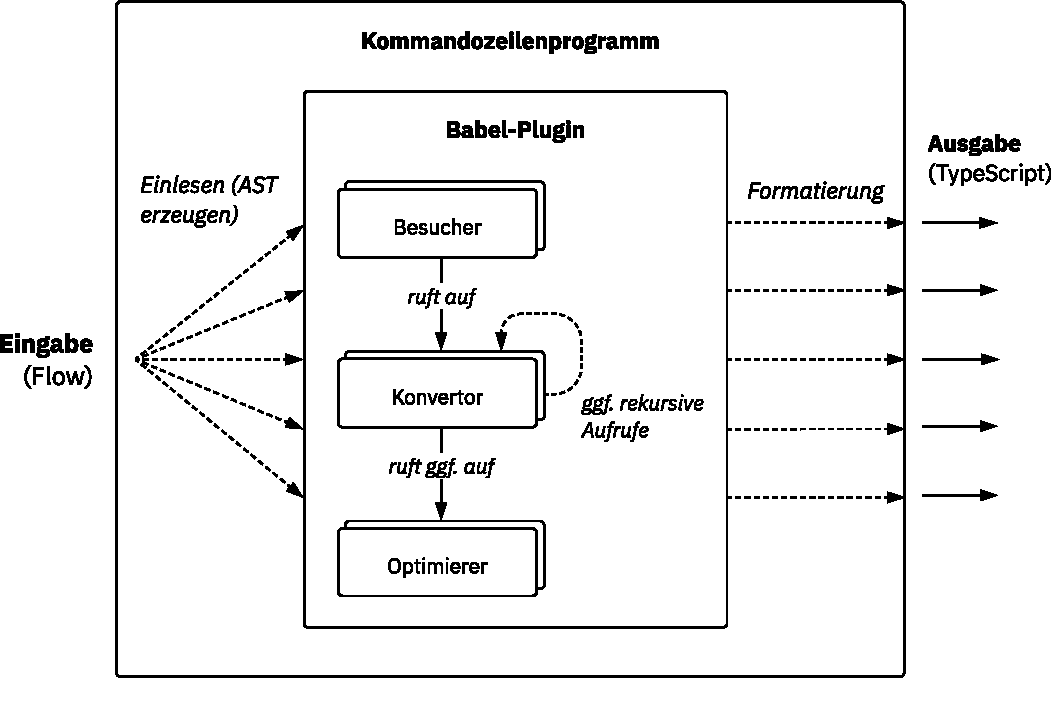
\includegraphics[width=\textwidth]{src/figures/architecture-overview.pdf}
        \end{figure}
      \end{columns}
    \end{frame}

    \begin{frame}
      \frametitle{Spezialfälle}
      TODO: Spezialfälle der Transformation
    \end{frame}

  \section{Ergebnisse}
    \secframe{3}{Ergebnisse und\\*\hspace{2.05em}Auswertung}

    \begin{frame}
      \frametitle{Durchführung der Migration}

    \end{frame}

    \begin{frame}
      \frametitle{Erkennung weiterer Typ- und Programmfehler}


    \end{frame}

    \begin{frame}
      \frametitle{TODO}

    \end{frame}

  \section{Zusammenfassung}
    \secframe{4}{Zusammenfassung}

    \begin{frame}
      \frametitle{TODO}

    \end{frame}

    \begin{frame}
      \frametitle{TODO}

    \end{frame}

  \appendix

    \begin{frame}[noframenumbering,plain]
      % empty
    \end{frame}

  \section{Anhang}
    \setbeamertemplate{footline}{}

    \begin{frame}[noframenumbering]
      \frametitle{Evaluation bestehender Werkzeuge}
      {
  \footnotesize
  \begin{tabu} to \textwidth {@{}lllccccccrrX@{}}
    \midrule
    Werkzeug & Typ & Format & Erw. & ES10 & ES10+ & Flow & TS & JSX \\
    \midrule
    Acorn     & P  &  ESTree  & \pie{2} & \pie{2} & \pie{1} & \pie{0} & \pie{0} & \pie{2} \\ % 2012
    Astring   & G  &  ESTree  & \pie{2} & \pie{2} & \pie{1} & \pie{0} & \pie{0} & \pie{0} \\ % 2015
    Babel     & PG &  Babel   & \pie{2} & \pie{2} & \pie{2} & \pie{2} & \pie{2} & \pie{2} \\ % 2014
    Escodegen & G  &  ESTree  & \pie{0} & \pie{0} & \pie{0} & \pie{0} & \pie{0} & \pie{0} \\ % 2012
    Esprima   & P  &  ESTree  & \pie{0} & \pie{1} & \pie{0} & \pie{0} & \pie{0} & \pie{1} \\ % 2011
    Recast    & PG &  diverse & \pie{2} & \pie{2} & \pie{2} & \pie{2} & \pie{2} & \pie{2} \\ % 2012
    \midrule
  \end{tabu}

  \vspace{5mm}
  \begin{columns}[T]
    \begin{column}{0.4\textwidth}
      {
        \renewcommand{\arraystretch}{1.1}
        \begin{tabular}{@{}ll@{}}
          P & Parser\\
          G & Codegenerator\\
          \pie{0} & keine Unterstützung\\
          \pie{1} & teilweise Unterstützung\\
          \pie{2} & vollständige Unterstützung\\
        \end{tabular}
      }
    \end{column}
    \begin{column}{0.5\textwidth}
      {
        \renewcommand{\arraystretch}{1.1}
        \begin{tabular}{@{}ll@{}}
          ES10 & ECMAScript 2019\\
          ES10+ & vorgeschlagene Spracherw.\\
          TS & TypeScript\\
        \end{tabular}
      }
    \end{column}
  \end{columns}
}

    \end{frame}

    \frame[allowframebreaks,noframenumbering,plain] {
      \frametitle{Quellenverzeichnis}
      \printbibliography
    }

\end{document}
